\documentclass[conference, 10pt]{IEEEtran}
%\IEEEoverridecommandlockouts
% The preceding line is only needed to identify funding in the first footnote. If that is unneeded, please comment it out.
\usepackage{cite}
\usepackage{amsmath,amssymb,amsfonts}
\usepackage{algorithmic}
\usepackage{graphicx}
\usepackage{textcomp}
\usepackage{xcolor}
\usepackage[colorlinks = true,
            linkcolor = blue,
            urlcolor  = blue,
            citecolor = blue,
            anchorcolor = blue]{hyperref}
\usepackage[spanish,activeacute]{babel}

\def\BibTeX{{\rm B\kern-.05em{\sc i\kern-.025em b}\kern-.08em
    T\kern-.1667em\lower.7ex\hbox{E}\kern-.125emX}}
\begin{document}

\title{Predicción del precio de bolsa de energía eléctrica Del Mercado Energía Mayorista Colombiano}

\author{\IEEEauthorblockN{Andrea Margarita Beleño}
\IEEEauthorblockA{200620739\\
E-mail:a.beleno@uniandes.edu.co}
\and
\IEEEauthorblockN{María Valeria Gaona}
\IEEEauthorblockA{202214418\\
E-mail:mv.gaona@uniandes.edu.co}
}

\maketitle

\begin{abstract}
El precio de bolsa de energía eléctrica del Mercado de Energía Mayorista (MEM) Colombiano está dado por diversos factores para generar un ambiente propicio de competencia y formación eficiente de precios, que le permitan a la demanda tener precios óptimos. Es por ello que es fundamental el análisis  de este mercado para que a medida que pase el tiempo, los agentes que participan en este mercado puedan identificar factores de riesgo más rápido y así, tomar las mejores decisiones para la economía y distribución de energía del país. Por lo tanto, de acuerdo con el análisis anterior, contar con una herramienta como una aplicación web que pueda predecir este valor genera una dinámica más eficiente para los agentes que están dentro del sector y a su vez, a ciudadanos que estén interesados en el campo energético. \
Para acceder a la aplicación web, se presenta el siguiente enlace: \url{https://aplicaciones-web-abeleno.shinyapps.io/pred_precio_bolsa_horario/} A su vez, el link al  repositorio del presente documento se encuentra en el siguiente enlace: \url{https://github.com/mvgaona/Proyecto-final-MEcA-4107}
\end{abstract}


\section{Introducción}
El mercado eléctrico colombiano es un mercado competitivo en donde participan generadores, transmisores, distribuidores, consumidores y comercializadores de energía. Este mercado se divide en dos segmentos: Corto y largo plazo, sin embargo, en el siguiente documento se presentará el análisis del mercado en corto plazo por medio de la bolsa de energía de Colombia, la cual es administrada por XM, en donde se presenta la participación de generadores y comercializadores de energía para la compra y venta a precio de bolsa de energía eléctrica, con el objetivo de suplir la demanda adecuada de energía en el país.\\
De acuerdo con Trespalacios, Pantoja \& Fernandez (2017)\cite{b5}, el mercado spot o la bolsa de energía hace referencia al mercado en donde se obtiene la energía eléctrica de forma instantánea, con el objetivo de lograr un balance entre oferta  y demanda. A su vez, los autores afirman que dicho precio de bolsa se define mediante un conjunto de normas que buscan precisar el nivel de referencia en caso de escasez.\\
Poveda (2012) \cite{b1} afirma que el despacho ideal es el programa de generación que está dado por el uso de los recursos más económicos hasta cubrir la demanda doméstica real, más las Transacciones Internacionales de Electricidad de Corto Plazo - TIE (Exportaciones como demanda e importaciones como generación), más las pérdidas del STN (Sistema de Transmisión Nacional). Teniendo en cuenta lo anterior, el precio de bolsa está dado por el precio de oferta obtenido por medio del despacho ideal, el cual es utilizado para valorar los intercambios en bolsa.\\
El correcto funcionamiento del mercado eléctrico es fundamental para el análisis de la demanda energética en el país: si es necesario realizar estrategias en el manejo de los recursos naturales con los que se genera energía, si la dinámica de compra y venta de energía está siendo óptima para la economía y sociedad colombiana. Generar una proyección de estos precios permite poder hacer inferencia acerca de cómo el mercado puede estar funcionando y aunque ´ este sea un sistema fluctuante, se puede generar predicciones acerca de su comportamiento.\\

En el siguiente documento se encuentra el análisis acerca de los datos recaudados para la predicción del precio de bolsa de energía eléctrica del mercado de energía mayorista colombiano, en donde se implementará un modelo de Machine Learning automático en una aplicación web, que permitirá modelar futuros precios de bolsa y con ello, tomar decisiones comerciales basadas en los datos adquiridos


\section{Datos} \label{AA}

El precio de bolsa de energía puede estar dado por diferentes factores que representan las condiciones del mercado energético colombiano, por ejemplo. Este precio se genera cada hora y, por lo tanto, es necesario considerar 24 modelos correspondientes a cada momento del día en donde se presentan cambios en este valor. Por lo tanto, para considerar realizar un modelo de predicción es necesario contar con factores determinantes que expliquen cómo se produce este precio. Por otra parte, dentro del análisis se recopiló información desde el 01/01/2000 hasta 30/06/2022, en donde no se presenta información faltante que deba ser imputada. En total la base cuenta con 8.217 observaciones.\\ 
Los datos a utilizar para el desarrollo de la predicción, se encuentran en la página del operador del mercado eléctrico colombiano XM. Esta empresa concentra todos los parámetros del sistema eléctrico colombiano que son importantes a la hora de realizar la predicción del precio de bolsa. Los predictores están dados por:\\
-\textit{Generación por tipo de recursos (kWh)}: Los recursos naturales permiten abastecer de energía eléctrica a las comunidades. Además, el precio de bolsa está representando por la generación de energía por medio de estos recursos, ya que esto permite que los agentes puedan continuar con su producción de energía y así, establecer dicho valor. Por lo tanto, existen 6 tipos de generadores: Eólica, solar, hidráulica, cogenerador y térmica.\\
Esta variable numérica cuenta con siguiente análisis descriptivo  de cada uno de los tipos de generadores. Como se observa en las siguientes gráficas, este análisis realizado para cada hora del día en el marco de fechas establecidas anteriormente.

-\textit{Índice Interoceánico de El Niño (ONI)}: Este indicador refleja la variación de la temperatura en el océano pacífico. Por lo tanto, al contar con un índice alto o mayor a 0.5 se presentan sequías, es decir, hay fenómeno del niño y si, por el contrario, el índice presenta valores pequeños o inferiores a -0.5 existe un fenómeno de la niña, en donde se presentan muchas lluvias. Por lo tanto, al presentarse el fenómeno del niño, los agentes generadores deben producir energía térmica, aumentando costos y llevando a que el precio de bolsa energético también aumente. Este indicador se da de manera mensual, se realizó la interpolación a datos diarios y se asume que es la misma para cada hora del día. Se obtuvo la información a través de web scrapping de la página web en \cite{b3}.\\

-\textit{Aportes totales (Aportes Hídricos en kWh)}: La variable representa cuanta energía se puede obtener de los ríos en Colombia. El precio de bolsa energético está altamente representado por esta variable ya que, la fuente principal energética del país es por medio del agua, ya que la matriz energética es 69\% hidráulica cite{b2}. Por lo tanto, Colombia depende de los ríos abastecer de energía a la sociedad. Es decir, a medida que aumenta el caudal en los ríos,el precio de bolsa disminuye. Este indicador se da de manera diaria, se asume que es la misma para cada hora del día.\\

-\textit{Tasa Representativa del mercado-TRM:} Este indicador hace referencia a la cantidad de pesos colombianos por un dólar estadounidense. Esta variable es relevante dentro de los modelos, debido a que el combustible térmico es pagado con la moneda dólar y por lo tanto, la variación de este valor genera un impacto, ya que estos recursos son distribuidos por medio de una moneda internacional, es decir, al contar con la moneda local devaluada, el precio de estos insumos aumenta. Este indicador se da de manera diaria, se asume que es la misma para cada hora del día.\\

Para las variables numéricas mencionadas anteriormente, se presenta la Figura ~\ref{fig_6} donde se encuentra el análisis descriptivo. 

\begin{figure}[htbp]
\centerline{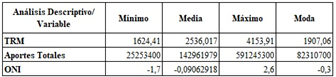
\includegraphics[width=0.5\textwidth]{../Images/Cuadro_descriptivo_varias_var.png}}
\caption{Cuadro descriptivo para TRM, ONI y Aportes totales}
\label{fig_6}
\end{figure}


\section{Modelo} \label{BB}

Con base en las variables presentadas en la sección \ref{AA}, se procedió a realizar, considerando series de tiempo, los modelos con diferentes hiperparámetros teniendo como base el \textit{XGBoost}. Se debe tener en cuenta, que el precio de bolsa del despacho ideal se da de manera horaria, por lo cual, se realizaron las predicciones para cada hora del día, considerando los predictores:\textit{TRM}, \textit{Aportes hídricos}, \textit{ONI}, la fecha (se dividió en \textit{año}, \textit{mes} y \textit{día} y el tipo de Generación (5 tipos de generación por 24 horas del día), dependiendo del recurso. Al ser series de tiempo los datos utilizados para desarrollar el presente trabajo, se dividió la base de datos en \textit{train} con el 70\% de los datos desde el 2000-01-01 y el restante 30\% fueron las fechas subsiguientes. Cabe anotar que para series de tiempo, las muestras de las bases a analizar deben ser secuenciales, por lo cual, dichas bases no se obtuvieron de manera aleatoria.\\
Ahora bien, se consideró que el modelo \textit{XGBoost} era el más apto para realizar la predicción del precio bolsa, teniendo en cuenta que este modelo se considera el mejor para aplicarlo a casos donde la no linealidad y la volatilidad son importantes. Se entrenaron varios modelos, de los cuales se presentan resultados de 2, en donde los hiperparámetros variaron para estos modelos para cada predicción del precio de bolsa para cada hora del día. Se explicará en breve los aspectos relevantes de cada modelo. Se debe tener en cuenta que para todos los modelos se utilizaron todas las variables contempladas en la sección \ref{AA}, es decir, 151 variables en total.

\begin{itemize}
\item \textit{\textbf{Modelo 1}}: Hiperparámetros importantes: $\lambda=0.3$ (tasa de aprendizaje), $d=3$ (número de bifurcaciones), $n=100$ (número de iteraciones). Esto se aplicó para la predicción del precio de bolsa horario para las 24 horas.
\item \item \textit{\textbf{Modelo 2}}: Hiperparámetros importantes: $\lambda=0.3$ (tasa de aprendizaje), $d=100$ (número de bifurcaciones), $n=1000$ (número de iteraciones). Esto se aplicó para la predicción del precio de bolsa horario para las 24 horas.
\end{itemize}

El parámetro de comparación entre modelos fue el RMSE. Para cada precio de bolsa horario se observó que los modelos presentados anteriormente, tenían diferente RMSE, tomándose el más bajo para realizar la predicción en la aplicación web. En el Cuadro ~\ref{tab_14} se presentan los resultados del RMSE para cada predicción de bolsa. En resumen, los precios de bolsa horarios a los cuales se les aplicó el modelo 1 o 2, se presentan a continuación: 

\begin{itemize}
\item \textit{\textbf{Modelo 1}}: Predicción del precio de bolsa para las horas: 0, 2, 3, 4, 5, 6, 7, 8, 9, 10, 12, 15, 17, 18, 22 y 23\item\textit{\textbf{Modelo 2}}: Predicción del precio de bolsa para las horas: 1, 11, 13, 14, 16, 19, 20 y 21.
\end{itemize}

Para el modelo 2, las horas predichas coinciden con las de mayor demanda en el sistema eléctrico colombiano. 

\subsection{Implementación en App web}
Ahora bien, para la implementación del modelo en la aplicación web, no fue necesario correr todo el código desarrollado en el modelo, sin embargo, para los predictores correspondientes a generación, se realizó una restricción de los datos a ingresar. Al tener los datos de las capacidades instaladas en generación del sistema (potencia), se obtuvo la suma de las capacidades de todos los generadores por tipo de generación, y así se obtuvo el rango en dichos predictores. Los resultados se muestran en el Cuadro ~\ref{tab_10}. No se puede asignar más capacidad de la que se encuentra instalada en el sistema de manera horaria.

\begin{table}[htbp]
\caption{Capacidades máximas en el SIN Colombiano por tipo de Generación}
\begin{center}
\begin{tabular}{|c|c|}
\hline
 Tipo de Generación&Capacidad (kW)\\
\hline 
Cogenerador&178.400\\
\hline
Eólica&20.000\\
\hline
Hidráulica&11.790.431\\
\hline
Térmica&8.823.450\\
\hline
Solar&157.726\\
  
	\hline
\end{tabular}
\label{tab_10}
\end{center}
\end{table}
  
\section{Resultados}
Para implementar el modelo en una aplicación web, utilizamos el paquete de \textit{Shiny} de R con los códigos especiales para que sean ejecutados mediante una página web. Para la implementación, se guardaron los modelos que menor RMSE tuvieron para cada modelo de precio horario y estos son los que se ejecutan en la página para la visualización e ingreso de variables por parte de un usuario. En la Figura ~\ref{fig_3} se muestra el entorno de la aplicación web de acceso público pero con limitación en el tiempo, con posibilidad de variar los campos a criterio y conocimiento del usuario, y después de unos segundos, se muestra el resultado de la aplicación. 

\begin{figure}[htbp]
\centerline{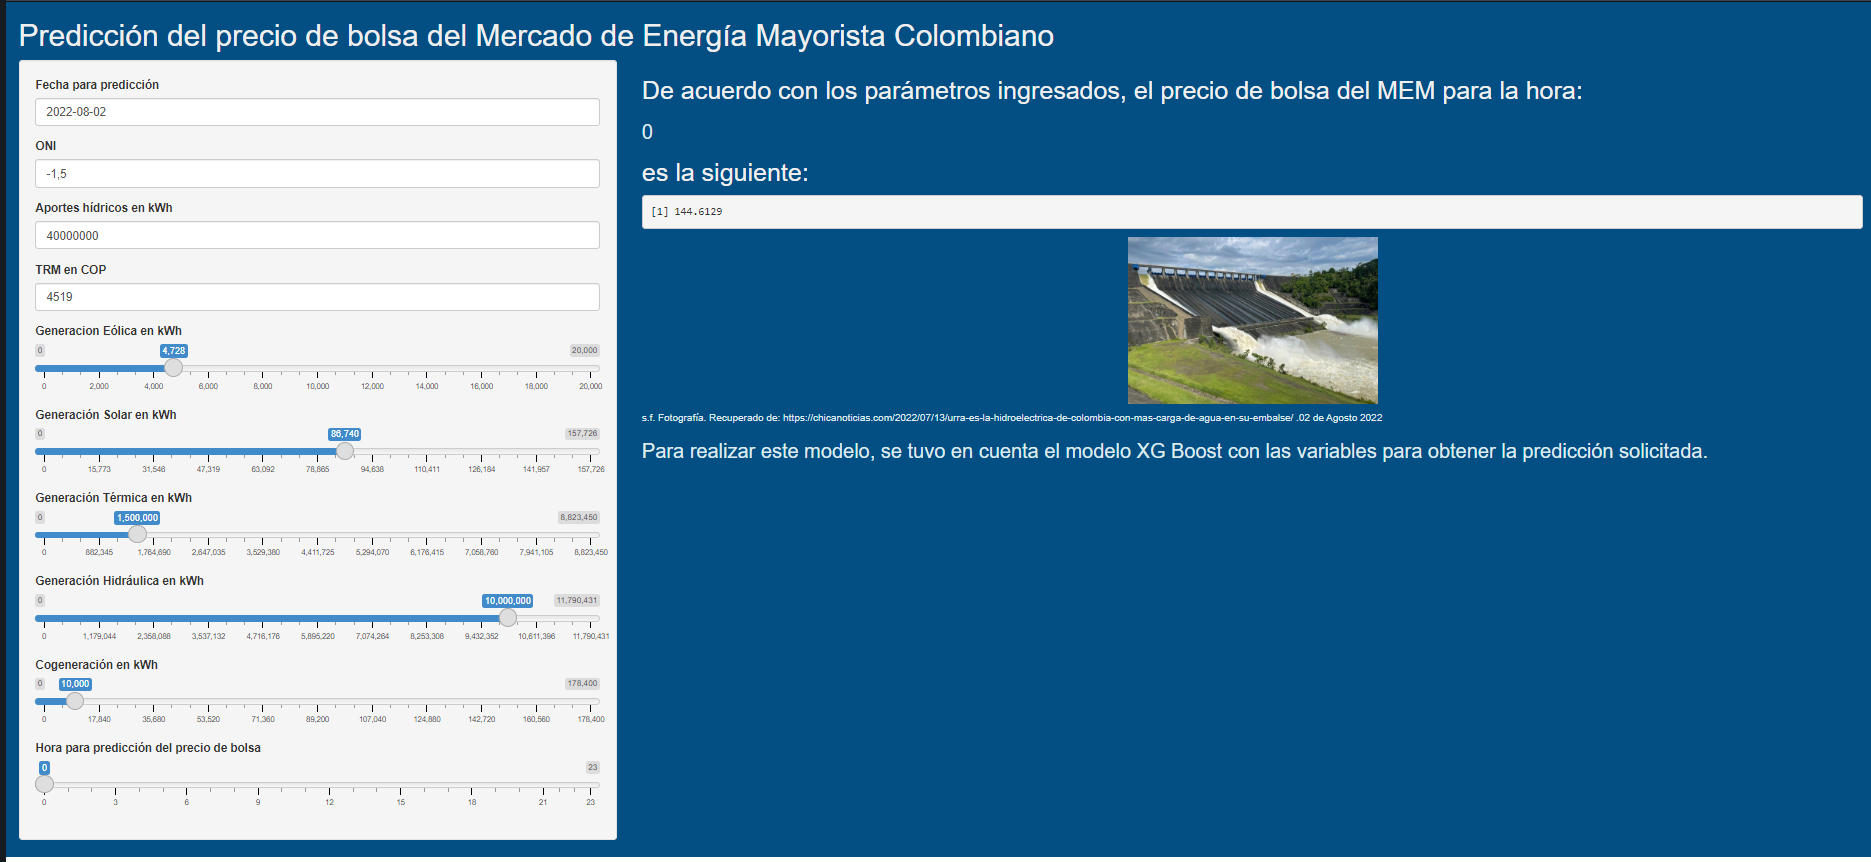
\includegraphics[width=0.5\textwidth]{../Images/Resultado_Trabajo_final.png}}
\caption{Resultado de la aplicación web}
\label{fig_3}
\end{figure}
De acuerdo con la aplicación web descrita anteriormente, cuyo enlace se encuentra en el abstract del presente documento, se presentan dos ejemplos de predicciones con diferentes valores reportados en las variables para Agosto 20\/2022 y Septiembre 10\/2022 en las Figuras ~\ref{fig_4}  y ~\ref{fig_5}, respectivamente.

\begin{figure}[htbp]
\centerline{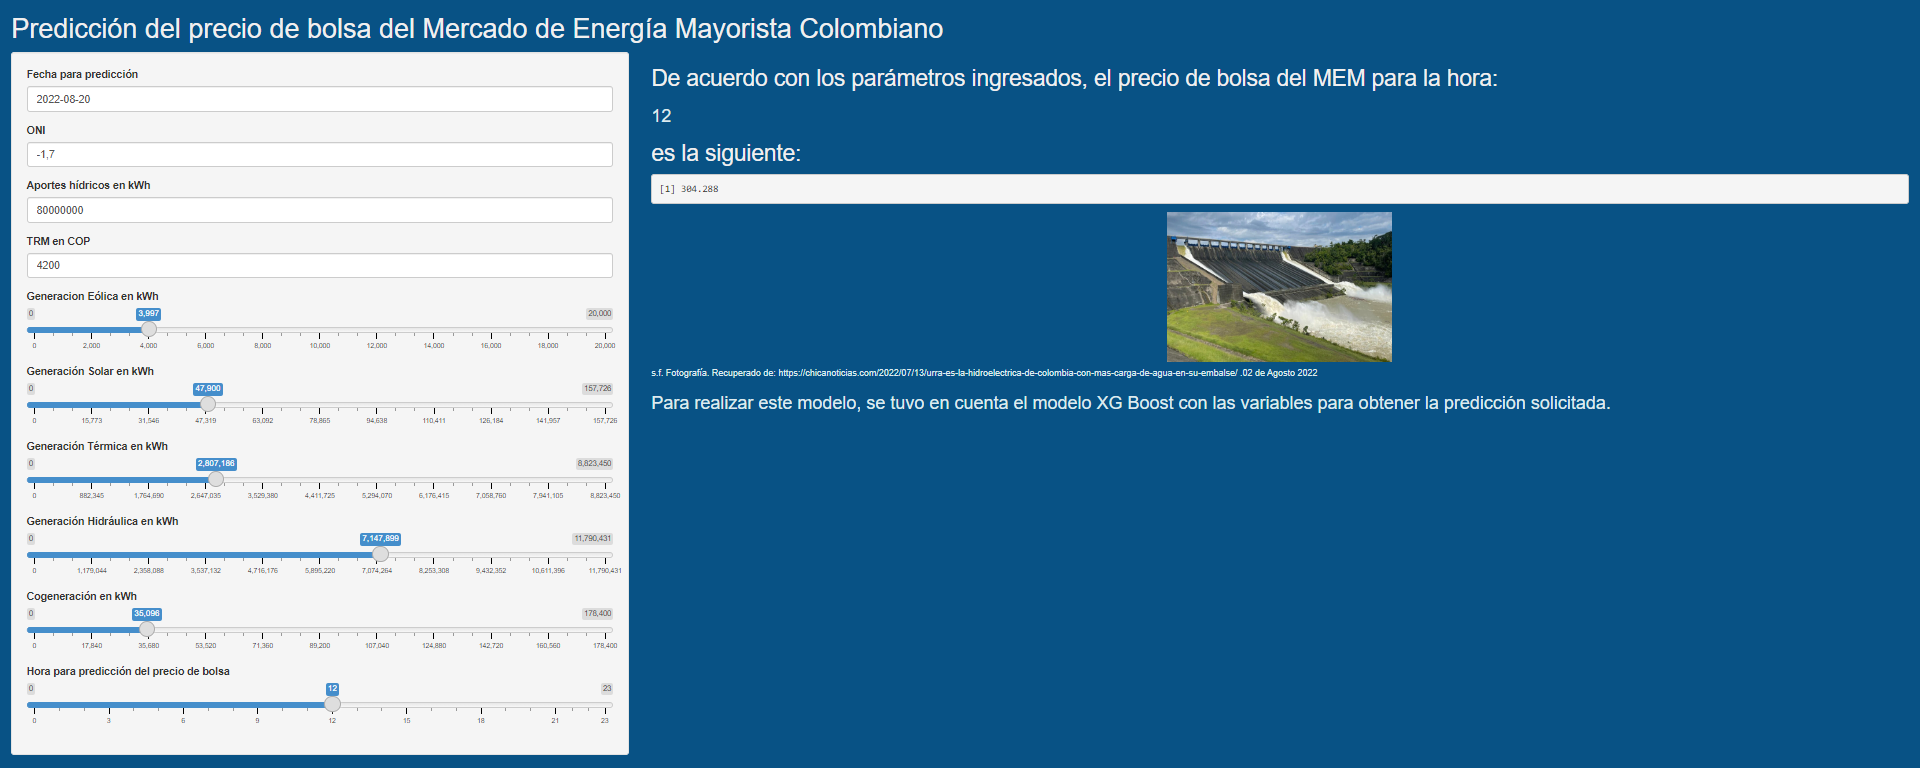
\includegraphics[width=0.5\textwidth]{../Images/AppWeb1.png}}
\caption{Ejemplo para Agosto 20/2022}
\label{fig_4}
\end{figure}


\begin{figure}[htbp]
\centerline{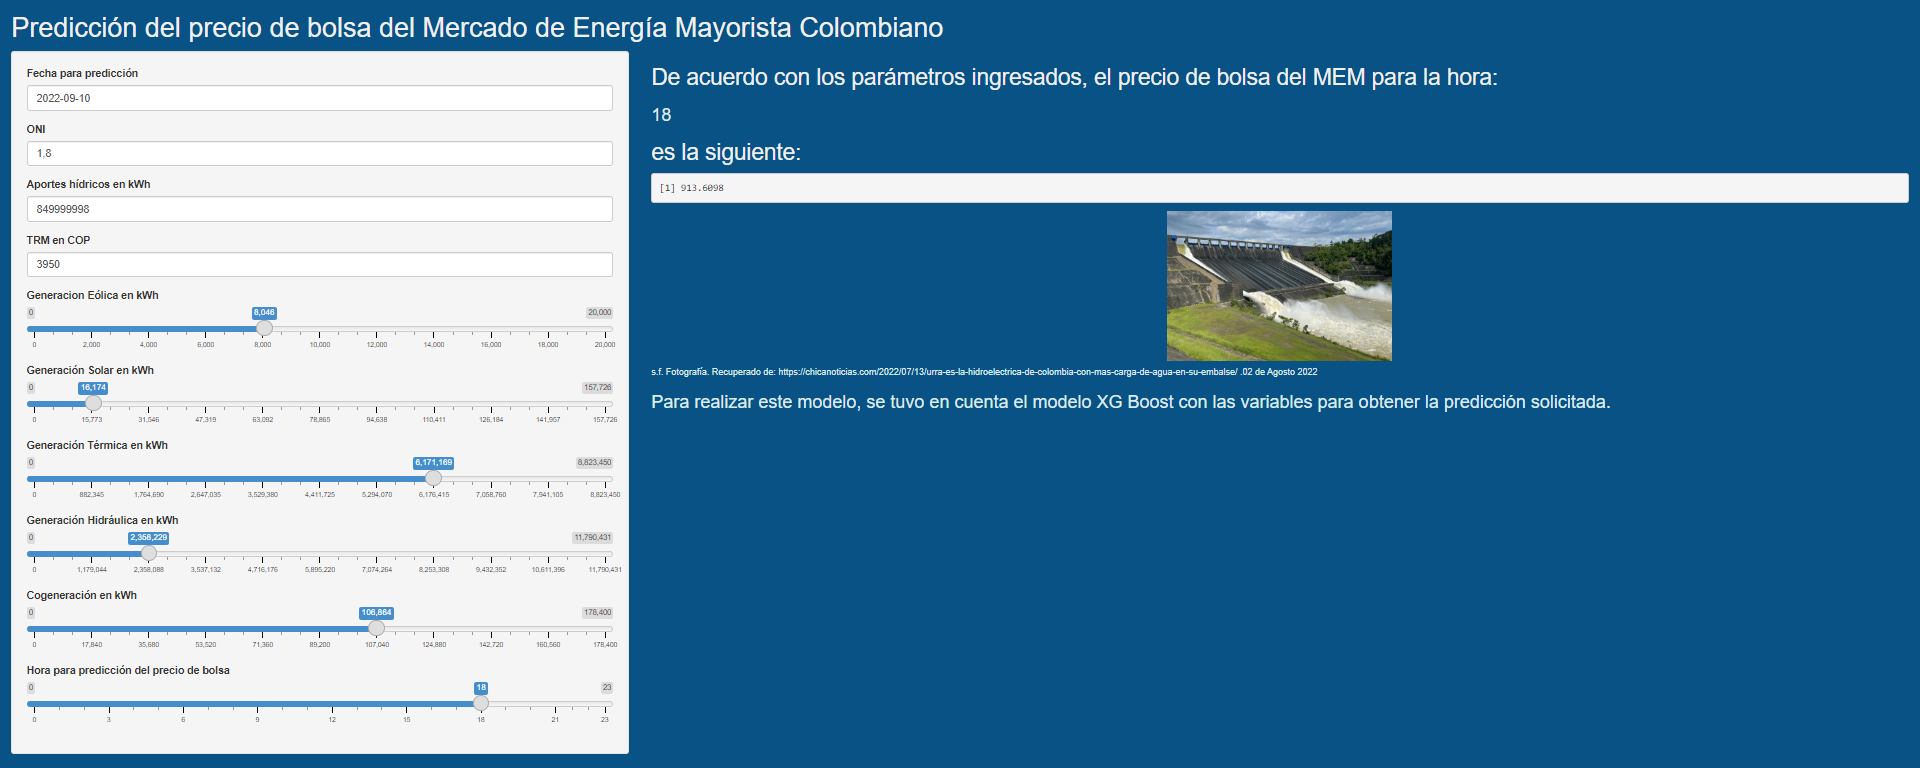
\includegraphics[width=0.5\textwidth]{../Images/AppWeb2.png}}
\caption{Ejemplo para Septiembre 10\/2022}
\label{fig_5}
\end{figure}



\section{Conclusiones y recomendaciones}
\begin{itemize}
\item Se encontró como limitación, que debido  a que el precio de bolsa energético es muy volátil y depende las ofertas en generación que realicen los agentes, se puede presentar algunas imprecisiones en la predicción de este valor, debido a que no fue posible disminuir el RMSE. 
Recomendaciones: Debido al hallazgo de la volatilidad de este precio, es necesario crear más estrategias que mitiguen este impacto volátil inevitable por medio de inclusión de diferentes más variables en los modelos por hora.

\item Fue un bastante interesante obtener los datos geográficos para utilizarlos como predictores o para imputar datos de variables existentes, fue en la parte del PS3 que más se demoró para obtener y que representó un gran reto y esfuerzo, sin embargo, consideramos la información obtenida muy relevante y que puede servir para futuras aplicaciones.
\item Los resultados más aceptables para el ejercicio fueron los que tuvieron en cuenta mayor cantidad de variables para obtener la predicción.
\item Para el presente trabajo, el modelo con menor RMSE y que también presentó una menor relación precio vs vivienda, fue el escogido para realizar la predicción y fue el que se entrenó posteriormente para obtener la predicción.
\item Como recomendación, con mayor cantidad de tiempo, se hubiese podido realizar otros modelos variando los hiperparámetros del modelo \textit{XGBoost}. 

\end{itemize}

\subsection{Recomendaciones}
\begin{itemize}
\item Debido al hallazgo de la volatilidad de este precio, es necesario crear más estrategias que mitiguen este impacto volátil inevitable por medio de inclusión de más variables en los modelos por hora, por ejemplo, los parámetros técnicos de los generadores (información no disponible de manera pública por parte de XM).

\item En cuanto a la Aplicación Web, se puede extender para que el usuario de la interfaz pueda escoger con qué otros modelos realice la predicción.

\end{itemize}

\begin{thebibliography}{00}
\bibitem{b1} Poveda Núñez, M. A. (2012) “Modelamiento del precio de bolsa. Universidad Nacional de Colombia.” Bogotá D.C, Recuperado de: \url{https://repositorio.unal.edu.co/bitstream/handle/unal/21159/300038.2012.pdf?sequence=1&isAllowed=y}
\bibitem{b2} XM (2022). Sinergox de XM. Recuperado de: \url{ https://sinergox.xm.com.co/trpr/Paginas/Historicos/Historicos.aspx.} 

\bibitem{b3}Climate Prediction Center.“Cold \& Warm episodes by season” Recuperado de: \url{https://origin.cpc.ncep.noaa.gov/products/analysis_monitoring/ensostuff/ONI_v5.php}

\bibitem{b4}XGBoost time series forecast in R.“xgboost time series forecast in R” Recuperado de: \url{http://datasideoflife.com/?p=1009#:~:text=xgboost\%2C\%20or\%20Extreme\%20Gradient\%20Boosting,while\%20doing\%20time\%20series\%20predictions.}

\bibitem{b5}Trespalacios Carrasquilla, A., Pantoja Robayo, J. O., \& Fernández Taborda, Ó. A. (2017). Análisis de mercados de electricidad. EAFIT.

\end{thebibliography}


\appendix[Cuadros de Variables descriptivas y RMSE]
Se presentan los Cuadros donde se consignan las estadísticas descriptivas de las variables explicadas en la sección \ref{AA} y \ref{BB} .\\ 


% Table created by stargazer v.5.2.3 by Marek Hlavac, Social Policy Institute. E-mail: marek.hlavac at gmail.com
% Date and time: mar., ago. 02, 2022 - 3:04:06 p. m.
\begin{table}[!htbp] \centering 
  \caption{Comparación de RMSE para modelo con bifurcación 3 y 100} 
  \label{} 
\begin{tabular}{@{\extracolsep{5pt}} ccc} 
\\[-1.8ex]\hline 
\hline \\[-1.8ex] 
Modelo & RMSE\_3 & RMSE\_100 \\ 
\hline \\[-1.8ex] 
Predicción\_h0 & $112.29$ & $141.76$ \\ 
Predicción\_h1 & $120.89$ & $119.11$ \\ 
Predicción\_h2 & $109.63$ & $112.36$ \\ 
Predicción\_h3 & $112.78$ & $115.21$ \\ 
Predicción\_h4 & $109.59$ & $115.15$ \\ 
Predicción\_h5 & $114.35$ & $127.95$ \\ 
Predicción\_h6 & $139.17$ & $146.15$ \\ 
Predicción\_h7 & $126.32$ & $133.02$ \\ 
Predicción\_h8 & $131.53$ & $138.11$ \\ 
Predicción\_h9 & $131.62$ & $136.65$ \\ 
Predicción\_h10 & $172.78$ & $217.50$ \\ 
Predicción\_h11 & $213.59$ & $201.64$ \\ 
Predicción\_h12 & $126.65$ & $137.01$ \\ 
Predicción\_h13 & $126.91$ & $124.82$ \\ 
Predicción\_h14 & $134.25$ & $129.88$ \\ 
Predicción\_h15 & $129.50$ & $135.12$ \\ 
Predicción\_h16 & $133.62$ & $130.76$ \\ 
Predicción\_h17 & $111.18$ & $125.89$ \\ 
Predicción\_h18 & $121.82$ & $141.82$ \\ 
Predicción\_h19 & $158.05$ & $136.94$ \\ 
Predicción\_h20 & $150.23$ & $136.19$ \\ 
Predicción\_h21 & $125.02$ & $120.78$ \\ 
Predicción\_h22 & $126.08$ & $151.35$ \\ 
Predicción\_h23 & $120.46$ & $132.46$ \\ 
\hline \\[-1.8ex] 
\end{tabular}
\label{tab_14} 
\end{table}


% Table created by stargazer v.5.2.3 by Marek Hlavac, Social Policy Institute. E-mail: marek.hlavac at gmail.com
% Date and time: mar., ago. 02, 2022 - 4:23:13 p. m.
\begin{table}[!htbp] \centering 
  \caption{Cuadro descriptivo para tipo de generación mediante Cogeneración} 
  \label{} 
\begin{tabular}{@{\extracolsep{5pt}} ccccc} 
\\[-1.8ex]\hline 
\hline \\[-1.8ex] 
Hora & Mín. & Máx. & Media & Moda \\ 
\hline \\[-1.8ex] 
h0 & 0 & 410.146 & 40.840,883 & 0 \\ 
h1 & 0 & 150.458,79 & 40.902,0432& 0 \\ 
h2 & 0 & 14.9261,96 & 41.014,700& 0 \\ 
h3 & 0 & 150.293,93 & 41.142,547& 0 \\ 
h4 & 0 & 147.386,04 & 41.050,650& 0 \\ 
h5 & 0 & 151.134,87 & 41.022,724& 0 \\ 
h6 & 0 & 152.285,89 & 40.554,742& 0 \\ 
h7 & 0 & 148.395,45 & 40.456,582& 0 \\ 
h8 & 0 & 145.334,36 & 40.113,777& 0 \\ 
h9 & 0 & 143.457,07 & 39.222,896& 0 \\ 
h10 & 0 & 141.100,67 & 38.617,483& 0 \\ 
h11 & 0 & 143.005,01 & 38.375,524& 0 \\ 
h12 & 0 & 148.322,67 & 38.565,889& 0 \\ 
h13 & 0 & 144.766,57 & 38.777,087& 0 \\ 
h14 & 0 & 143.230,34 & 38.465,044& 0 \\ 
h15 & 0 & 142.148 & 38.513,413& 0 \\ 
h16 & 0 & 145.504,87 & 38.936,497& 0 \\ 
h17 & 0 & 144.053,28 & 39.410,824& 0 \\ 
h18 & 0 & 138.961,56 & 39.291,810& 0 \\ 
h19 & 0 & 145.042,94 & 39.659,454& 0 \\ 
h20 & 0 & 142.540,31 & 40.354,904& 0 \\ 
h21 & 0 & 144.540,66 & 40.660,369& 0 \\ 
h22 & 0 & 146.768,19 & 40.348,729& 0 \\ 
h23 & 0 & 143.285,56 & 40.450,315& 0 \\ 
\hline \\[-1.8ex] 
\end{tabular} 
\label{tab_15}
\end{table}


% Table created by stargazer v.5.2.3 by Marek Hlavac, Social Policy Institute. E-mail: marek.hlavac at gmail.com
% Date and time: mar., ago. 02, 2022 - 4:24:24 p. m.
\begin{table}[!htbp] \centering 
  \caption{Cuadro descriptivo para tipo de generación Hidráulica} 
  \label{} 
\begin{tabular}{@{\extracolsep{5pt}} ccccc} 
\\[-1.8ex]\hline 
\hline \\[-1.8ex] 
Hora & Mín. & Máx. & Media & Moda \\ 
\hline \\[-1.8ex] 
h0 & 1.417.548,91 & 7.628.404,46 & 4.528.715,493& 1.417.548,91 \\ 
h1 & 1.330.047,13 & 7.647.431,1 & 4.398.223,237& 1.330.047,13 \\ 
h2 & 1.324.454,7 & 7.557.410,8 & 4.298.109,397& 1.324.454,7 \\ 
h3 & 1.283.247,27 & 7.416.477,69 & 4.268.356,919& 1.283.247,27 \\ 
h4 & 1.183.501,72 & 7.536.784,76 & 4.424.014,275& 1.183.501,72 \\ 
h5 & 1.179.017,14 & 7.833.471,26 & 4.822.082,199& 5.570.182,61 \\ 
h6 & 970.812,04 & 8.091.892,65 & 4.993.436,200& 3.995.987,35 \\ 
h7 & 1.306.117,5 & 8.618.320,45 & 5.303.482,864& 1.306.117,5 \\ 
h8 & 1.664.275,94 & 9.178.610,74 & 5.705.667,277& 1.664.275,94 \\ 
h9 & 1.806.851,95 & 9.442.061,34 & 5.952.079,715& 1.806.851,95 \\ 
h10 & 92.118,27 & 9.678.024,4 & 6.185.775,403& 92.118,27 \\ 
h11 & 765.668,02 & 9.986.122,45 & 6.352.912,141& 765.668,02 \\ 
h12 & 2.129.648,15 & 9.975.165,45 & 6.200.989,860& 2.129.648,15 \\ 
h13 & 1.335.052,8 & 9.983.786,18 & 6.103.800,306& 1.335.052,8 \\ 
h14 & 1.970.576,06 & 10.130.255,68 & 6.110.836,725& 1.970.576,06 \\ 
h15 & 1.795.877,68 & 10.060.447,37 & 6.074.021,695& 1.795.877,68 \\ 
h16 & 1.666.592,38 & 9.927.489,34 & 6.007.630,163& 1.666.592,38 \\ 
h17 & 1.268.806,53 & 9.897.813,48 & 6.063.786,198& 5.633.259,81 \\ 
h18 & 2.612.639,5 & 10.322.512,92 & 6.978.153,396& 2.612.639,5 \\ 
h19 & 3.529.632,31 & 10.401.510,03 & 7.246.731,128& 3.529.632,31 \\ 
h20 & 3.350.340,67 & 10.158.243,39 & 6.938.421,981& 3.350.340,67 \\ 
h21 & 2.478.786,26 & 9.737.813,23 & 6.401.386,069& 2.478.786,26 \\ 
h22 & 1.888.084,34 & 9.148.863,62 & 5.656.073,321& 1.888.084,34 \\ 
h23 & 1.106.884,57 & 8.589.358,18 & 4.989.189,830& 1.106.884,57 
\\ \hline \\[-1.8ex] 
\end{tabular} 
\label{tab_16}
\end{table}

% Table created by stargazer v.5.2.3 by Marek Hlavac, Social Policy Institute. E-mail: marek.hlavac at gmail.com
% Date and time: mar., ago. 02, 2022 - 4:26:49 p. m.
\begin{table}[!htbp] \centering 
  \caption{Cuadro descriptivo para tipo de generación térmica} 
 
\begin{tabular}{@{\extracolsep{5pt}} ccccc} 
\\[-1.8ex]\hline 
\hline \\[-1.8ex] 
Hora & Mín. & Máx. & Media & Moda \\ 
\hline \\[-1.8ex] 
h0 & 0 & 4.346.958,35 & 952.843,162& 0 \\ 
h1 & 0 & 4.376.783,85 & 866.869,172& 0 \\ 
h2 & 0 & 4.389.886,65 & 842.063,152& 0 \\ 
h3 & 0 & 4.402.622,4 & 836.680,849& 0 \\ 
h4 & 0 & 4.400.095,75 & 850.738,131& 0 \\ 
h5 & 0 & 4.400.159,45 & 874.619,085& 0 \\ 
h6 & 0 & 4.396.572,75 & 888.079,991& 0 \\ 
h7 & 0 & 4.392.592,85 & 908.524,226& 0 \\ 
h8 & 0 & 4.397.880,86 & 9.30.736,171& 0 \\ 
h9 & 0 & 4.381.757 & 942.592,613& 0 \\ 
h10 & 0 & 4.284.917,55 & 954.549,728& 150.000 \\ 
h11 & 0 & 4.248.899,11 & 966.628,179& 150.000 \\ 
h12 & 0 & 4.263.505,75 & 966.729,394 & 150.000 \\ 
h13 & 0 & 4.272.879,6 & 965.323,129& 150.000 \\ 
h14 & 0 & 4.375.807,45 & 967.056,145 & 150.000 \\ 
h15 & 0 & 4.391.872,75 & 968.643,591 & 150000 \\ 
h16 & 0 & 4.394.330,1 & 972.772,873 & 150000 \\ 
h17 & 0 & 4.397.210,45 & 989.960,17 & 150000 \\ 
h18 & 0 & 4.399.168,6 & 1.023.728,482& 150000 \\ 
h19 & 0 & 4.405.031,2 & 1.040.641,069 & 150000 \\ 
h20 & 0 & 4.409.350,3 & 1.022.014,044 & 150000 \\ 
h21 & 0 & 4.415.668,25 & 996.256,082 & 150000 \\ 
h22 & 0 & 4.387.023,65 & 958.256,776 & 150000 \\ 
h23 & 0 & 4.379.308,16 & 918.575,431 & 0 \\ 
\hline \\[-1.8ex] 
\end{tabular} 
\label{tab_17}
\end{table}

% Table created by stargazer v.5.2.3 by Marek Hlavac, Social Policy Institute. E-mail: marek.hlavac at gmail.com
% Date and time: mar., ago. 02, 2022 - 4:28:02 p. m.
\begin{table}[!htbp] \centering 
  \caption{Cuadro descriptivo para tipo de generación solar} 
  \label{} 
\begin{tabular}{@{\extracolsep{5pt}} ccccc} 
\\[-1.8ex]\hline 
\hline \\[-1.8ex] 
Hora & Mín. & Máx. & Media & Moda \\ 
\hline \\[-1.8ex] 
h0 & 0 & 479,26 & 0,159& 0 \\ 
h1 & 0 & 471,58 & 0,155& 0 \\ 
h2 & 0 & 459,8 & 0,152& 0 \\ 
h3 & 0 & 450,15 & 0,151& 0 \\ 
h4 & 0 & 461,67 & 0,157& 0 \\ 
h5 & 0 & 940,49 & 11,715 & 0 \\ 
h6 & 0 & 48.263,35 & 1.270,431& 0 \\ 
h7 & 0 & 122.211,63 & 5.003,544& 0 \\ 
h8 & 0 & 139.131,62 & 8.256,382& 0 \\ 
h9 & 0 & 164.277,33 & 10.391,743& 0 \\ 
h10 & 0 & 167.135,36 & 11.581,421& 0 \\ 
h11 & 0 & 175.221,75 & 12.069,044& 0 \\ 
h12 & 0 & 164.512,27 & 11.996,089& 0 \\ 
h13 & 0 & 164.651,47 & 11.402,893& 0 \\ 
h14 & 0 & 154.896,74 & 10.246,819& 0 \\ 
h15 & 0 & 140.096,57 & 8.208,544& 0 \\ 
h16 & 0 & 993.22,75 & 4.685,860& 0 \\ 
h17 & 0 & 25.263,59 & 834,022& 0 \\ 
h18 & 0 & 5.485,35 & 3,113& 0 \\ 
h19 & 0 & 520,83 & 0,219& 0 \\ 
h20 & 0 & 468,67 & 0,166& 0 \\ 
h21 & 0 & 466,98 & 0,178& 0 \\ 
h22 & 0 & 468,25 & 0,162& 0 \\ 
h23 & 0 & 469,52 & 0,160& 0 \\ \hline \\[-1.8ex] 
\end{tabular} 
\label{tab_18}
\end{table}


% Table created by stargazer v.5.2.3 by Marek Hlavac, Social Policy Institute. E-mail: marek.hlavac at gmail.com
% Date and time: mar., ago. 02, 2022 - 4:29:02 p. m.
\begin{table}[!htbp] \centering 
  \caption{Cuadro descriptivo para tipo de generación eólica} 
  \label{} 
\begin{tabular}{@{\extracolsep{5pt}} ccccc} 
\\[-1.8ex]\hline 
\hline \\[-1.8ex] 
Hora & Mín. & Máx. & Media & Moda \\ 
\hline \\[-1.8ex] 
h0 & 0 & 16.557,13 & 3.366,288& 0 \\ 
h1 & 0 & 16.074,14 & 3.146,872& 0 \\ 
h2 & 0 & 16.136,39 & 2.961,920& 0 \\ 
h3 & 0 & 15.162,08 & 2.810,429& 0 \\ 
h4 & 0 & 15.586,59 & 2.656,932& 0 \\ 
h5 & 0 & 15.242,7 & 2.550,637& 0 \\ 
h6 & 0 & 16.500,46 & 2.574,470& 0 \\ 
h7 & 0 & 16.616,68 & 3.010,651& 0 \\ 
h8 & 0 & 16.917,75 & 3.463,020& 0 \\ 
h9 & 0 & 17.026,27 & 3.819,577& 0 \\ 
h10 & 0 & 17.680,5 & 4.338,920& 0 \\ 
h11 & 0 & 17.564,76 & 5.181,301& 0 \\ 
h12 & 0 & 17.660,44 & 6.227,226& 0 \\ 
h13 & 0 & 17.989,05 & 7.006,291& 0 \\ 
h14 & 0 & 18.423,85 & 7.549,247& 0 \\ 
h15 & 0 & 18.345,76 & 7.841,002& 0 \\ 
h16 & 0 & 17.863,57 & 7.736,863& 0 \\ 
h17 & 0 & 17.865,31 & 7.151,004& 0 \\ 
h18 & 0 & 17.896,9 & 6.101,1048& 0 \\ 
h19 & 0 & 17.346,61 & 5.195,802& 0 \\ 
h20 & 0 & 17.366,73 & 4.618,033& 0 \\ 
h21 & 0 & 17.777,47 & 4.226,125& 0 \\ 
h22 & 0 & 17.365,74 & 3.903,933& 0 \\ 
h23 & 0 & 17.181,65 & 3.624,142& 0 \\ 
\hline \\[-1.8ex] 
\end{tabular} 
\label{tab_19}
\end{table}







\end{document}
